\documentclass[14pt,letterpaper]{extarticle}
\usepackage[margin=0.65in,top=0.8in,bottom=0.72in]{geometry}
\usepackage{tikz}
\usepackage{array}
\usepackage{fancyhdr}
\usepackage[T1]{fontenc}
\usepackage{helvet}
\renewcommand{\familydefault}{\sfdefault}
\setlength{\parindent}{0pt}
\setlength{\parskip}{9pt}
\setlength{\headheight}{16pt}
\setlength{\headsep}{14pt}
\pagestyle{fancy}
\fancyhf{}
\renewcommand{\headrulewidth}{0.3pt}
\renewcommand{\footrulewidth}{0pt}
\fancyfoot[L]{\fontsize{10}{12}\selectfont Bellingham Math Circle / Week 11 / F11-RV-v1}
\fancyfoot[R]{\fontsize{10}{12}\selectfont\thepage}
\newcommand{\band}[1]{\fancyhead[L]{\fontsize{12}{14}\selectfont Week 11 / Chip firing / #1}}
\newcommand{\prob}[2]{\textbf{Problem #1:} #2}
\newcommand{\wordexample}{%
\begin{tikzpicture}[x=1cm,y=1cm,line width=0.65pt]
 \foreach \offset/\caption in {0/Before,5/{A fires},10/After}{%
   \begin{scope}[shift={(\offset,0)}]
   \draw (0,0)--(1.7,0)--(.85,1.3)--cycle;
   \foreach \x/\y/\lab/\tx/\ty in {0/0/A/-.58/0,1.7/0/B/2.28/0,.85/1.3/C/.85/1.9}{%
     \draw[fill=white] (\x,\y) circle[radius=.38cm];
     \node[font=\small] at (\tx,\ty) {\lab};
   }
   \node[font=\small] at (.85,2.45) {\caption};
   \end{scope}
 }
 \fill (-.14,0) circle[radius=.075cm];
 \fill (.14,0) circle[radius=.075cm];
 \draw[->,line width=1pt] (5.43,0)--(6.26,0);
 \draw[->,line width=1pt] (5.23,.35)--(5.64,.98);
 \fill (5.78,0) circle[radius=.075cm];
 \fill (5.40,.61) circle[radius=.075cm];
 \fill (11.7,0) circle[radius=.075cm];
 \fill (10.85,1.3) circle[radius=.075cm];
 \node[font=\small] at (10.85,-.7) {Word: A};
\end{tikzpicture}}
\newcommand{\closedboard}{%
\begin{tikzpicture}[x=1cm,y=1cm,line width=1.2pt]
 \draw (0,0)--(6,0)--(3,5.2)--cycle;
 \foreach \x/\y/\lab/\tx/\ty in {0/0/A/-2.42/0,6/0/B/8.42/0,3/5.2/C/3/7.6}{%
   \draw[fill=white] (\x,\y) circle[radius=2.1cm];
   \node[font=\large] at (\tx,\ty) {\lab};
 }
\end{tikzpicture}}
\newcommand{\cycleboard}{%
\begin{tikzpicture}[x=1cm,y=1cm,line width=1.2pt]
 \draw (0,0)--(5.8,0)--(5.8,5.8)--(0,5.8)--cycle;
 \foreach \x/\y/\lab/\tx/\ty in {0/0/A/-2.42/0,5.8/0/B/8.22/0,5.8/5.8/C/8.22/5.8}{%
   \draw[fill=white] (\x,\y) circle[radius=2.1cm];
   \node[font=\large] at (\tx,\ty) {\lab};
 }
 \draw[fill=white] (0,5.8) circle[radius=2.75cm];
 \node[font=\large] at (0,5.8) {Sink};
\end{tikzpicture}}
\newcommand{\sinktriangle}{%
\begin{tikzpicture}[x=1cm,y=1cm,line width=1.2pt]
 \draw (0,0)--(6,0)--(3,5.2)--cycle;
 \foreach \x/\y/\lab/\tx/\ty in {0/0/A/-2.42/0,6/0/B/8.42/0}{%
   \draw[fill=white] (\x,\y) circle[radius=2.1cm];
   \node[font=\large] at (\tx,\ty) {\lab};
 }
 \draw[fill=white] (3,5.2) circle[radius=2.75cm];
 \node[font=\large] at (3,5.2) {Sink};
\end{tikzpicture}}
\begin{document}
\band{K--1 and Grades 2--3}
\setlength{\parskip}{4pt}
\setlength{\topsep}{4pt}
Choose one circle at a time. It can fire when it has at least one chip for each line from it. Send one chip from it along each line. A sink never fires; chips there stay. Write the firing circle's letter after each move.

\begin{center}\wordexample\end{center}

\prob{1}{Try these starts. Which can stop with no circle able to fire? Which can return to an earlier position?}

\begin{center}
\renewcommand{\arraystretch}{1.1}
\begin{tabular}{|c|c|c|}\hline
Start 1 & Start 2 & Start 3\\\hline
\strut A: 3, B: 0, C: 0 & A: 2, B: 1, C: 0 & A: 4, B: 0, C: 0\\\hline
\end{tabular}
\end{center}
\begin{center}\closedboard\end{center}
\renewcommand{\arraystretch}{1.25}
\begin{tabular}{|p{0.6in}|p{3.6in}|p{1.8in}|}\hline
Start & Firing letters, in order & Finish or repeat\\\hline
1 & & \\\hline
2 & & \\\hline
3 & & \\\hline
\end{tabular}

\newpage
\band{Grades 2--3 and 4--5}
\setlength{\parskip}{9pt}
\prob{2}{Put one chip at each of A, B and C. Add one chip at A, B or C, then fire until no circle can fire. For each trial, restore the chosen starting piles and empty the sink before adding a chip. Among all starts with at most one chip at each of A, B and C, which start and added chip make the longest firing word?}

\begin{center}\cycleboard\end{center}
\vspace{0.03in}
\renewcommand{\arraystretch}{1.62}
\begin{tabular}{|p{1.18in}|p{0.66in}|p{2.47in}|p{1.52in}|}\hline
Start\newline A, B, C & Add at & Firing letters, in order & Finish\newline A, B, C\\\hline
1, 1, 1 & A & & \\\hline
1, 1, 1 & B & & \\\hline
1, 1, 1 & C & & \\\hline
 & & & \\\hline
 & & & \\\hline
 & & & \\\hline
\end{tabular}

\newpage
\band{Grades 4--5}
\prob{3}{Each start below can finish with one chip at A, one at B and four in the sink, using exactly four firings. The sink starts empty. Find every legal four-letter firing word for each start.}

\begin{center}\sinktriangle\end{center}
\vspace{0.08in}
\renewcommand{\arraystretch}{1.64}
\begin{tabular}{|p{1.45in}|p{4.6in}|}\hline
Start: A, B & Legal four-letter firing words\\\hline
0, 6 & \rule{0pt}{.75in}\\\hline
3, 3 & \rule{0pt}{.75in}\\\hline
6, 0 & \rule{0pt}{.75in}\\\hline
\end{tabular}
\end{document}
